% test change
\documentclass[10pt,a4paper]{article}

% --- Page + typography (matches the look of the screenshot) ---
\usepackage[a4paper,margin=0.55in]{geometry}
\usepackage[T1]{fontenc}
\usepackage[utf8]{inputenc}
\usepackage{newtxtext} % Times-like
\usepackage{microtype}
\usepackage{xcolor}
\usepackage[final]{graphicx} % force real images (avoid draft placeholders)
\usepackage{tabularx}
\usepackage{array}
\usepackage{enumitem}
\usepackage{xurl} % nicer URL line breaks
\usepackage[hidelinks]{hyperref}
\urlstyle{same}

\pagestyle{empty}
\setlength{\parindent}{0pt}
\setlength{\parskip}{0pt}

% --- Colors / rules ---
\definecolor{Accent}{HTML}{1F4E79}

\newcommand{\sectionrule}{\par\vspace{3pt}{\color{Accent}\hrule height 1pt}\vspace{3pt}}
\newcommand{\Section}[1]{%
  {\sectionrule \color{Accent}\bfseries\uppercase{#1}}\par\sectionrule
}

% --- Lists (tight bullets like the screenshot) ---
\setlist[itemize]{
  leftmargin=1.1em,
  topsep=1pt,
  itemsep=1pt,
  parsep=0pt,
  partopsep=0pt
}
\renewcommand{\labelitemi}{\textbullet}

% --- Entry row: left title/company + right date ---
\newcolumntype{L}{>{\raggedright\arraybackslash}X}
\newcolumntype{R}{>{\raggedleft\arraybackslash}p{0.34\linewidth}}
\newcommand{\WorkEntry}[3]{%
  \begin{tabularx}{\linewidth}{@{}L R@{}}
    {\bfseries #1 \textbar\  #2} & {\footnotesize\itshape\sloppy #3}\\
  \end{tabularx}
}

\begin{document}

% ---------------- Header ----------------
\begin{minipage}[t]{0.80\linewidth}
{\color{Accent}\bfseries\LARGE POTLURI KRISHNA PRIYATHAM}\par
{\large \bfseries Software Engineer \textbullet\ AI/ML/Data Practitioner \textbullet\ Quantum Computing Enthusiast}\par
\vspace{3pt}
% Removed \small from this section to increase URL size and fill horizontal space
\large
\href{mailto:kittu.priyatham@gmail.com}{\nolinkurl{kittu.priyatham@gmail.com}} \textbar\
\href{https://www.linkedin.com/in/potluri-krishna-priyatham}{\nolinkurl{linkedin.com/in/potluri-krishna-priyatham}}\\
\href{https://github.com/kittupriyatham}{\nolinkurl{github.com/kittupriyatham}} \textbar\
\href{https://www.stopstalk.com/user/profile/kittu_priyatham}{\nolinkurl{stopstalk.com/user/profile/kittu_priyatham}}\\
\href{https://potluri-krishna-priyatham.tech}{\nolinkurl{potluri-krishna-priyatham.tech}} \textbar\
\href{https://credly.com/users/potluri-krishna-priyatham}{\nolinkurl{credly.com/users/potluri-krishna-priyatham}}\par
\end{minipage}
\hfill
\begin{minipage}[t]{0.18\linewidth}
\raggedleft
\vspace*{-10pt} % Use a negative value to pull the image up
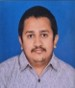
\includegraphics[width=2.5cm]{mypic.png}
\end{minipage}

\vspace{0pt}

% ---------------- Summary ----------------
\par
\Section{Summary}
{
Problem solver, software engineer and AI/ML/Data practitioner with \textasciitilde{}2 years of industry experience across defence systems (BEL), enterprise mobile (Jio Platforms), and cloud-deployed ML applications. Skilled across full-stack development, data science, and quantum computing. Known for breaking down ambiguous requirements, identifying root causes, and delivering reliable solutions with hands-on cloud deployment, system design/architecture, and autonomous AI agent experience.
}

\vspace{4pt}

% ---------------- Skills ----------------
\Section{Skills}
{\small
\textbf{Quantum:} Qiskit, Cirq, QBraid, Azure Quantum\\
\textbf{Mathematics:} Linear Algebra, Probability, Numerical Methods, Advanced Calculus\\
\textbf{Languages:} Python, Java, C/C++, JavaScript, Swift, SQL, HTML/CSS\\
\textbf{Frameworks \& ML:} Spring Boot, React, Flask, TensorFlow, PyTorch, Scikit-Learn, LangChain, OpenCV, Pandas, NumPy\\
\textbf{Cloud \& Other Tools:} AWS, Azure, MySQL, MongoDB, PostgreSQL, Power BI, Git, Docker
}\par

\vspace{4pt}

% ---------------- Work Experience ----------------
\Section{Work Experience}

\WorkEntry{Deputy Engineer}{Bharat Electronics Limited (BEL)}{Jun 2025 -- Mar 2026}
\begin{itemize}
  \item Contributed to the AEW\&C Maintenance Management System (Java Spring Boot, React, Python) by implementing key modules and proposing an OCR-based document ingestion flow to auto-fill forms and surface extracted fields --- estimated to reduce manual data entry by \textasciitilde{}68\%.
  \item Engineered a high-reliability Ventilator System UI with Qt/QML meeting strict safety standards.
  \item Designed and engineered the VAAMS system architecture, defining key modules and integration points across software and hardware components.
\end{itemize}

\WorkEntry{Software Intern}{Jio Platforms Limited}{Aug 2022 -- Jul 2023}
\begin{itemize}
  \item Engineered 5+ major features and resolved 20+ critical bugs for the JioMeet macOS client, driving a 35\% increase in app performance and significantly enhancing the end-to-end user experience for millions of users.
  \item Ensured platform stability and data continuity by upgrading to GA4 tracking and maintaining high-quality Swift/Objective-C codebases, resulting in a 99.9\% session success rate across the platform.
\end{itemize}

\WorkEntry{ML Intern}{Indian Servers}{Jun 2021 -- Aug 2021}
\begin{itemize}
  \item Built and deployed IRIS flower classification ML model (Scikit-learn + Flask) on Azure App Service with 90\% model accuracy.
\end{itemize}

\vspace{2pt}

% ---------------- Projects ----------------
\Section{Projects}

\WorkEntry{Own Agent --- Personal AI Agent}{LangChain, Gemini, Python}{\href{https://github.com/kittupriyatham/OwnAgent}{github.com/kittupriyatham/OwnAgent}}
\begin{itemize}
  \item Autonomous agent executing system tasks, file operations, and real-time web research through a custom toolset.
\end{itemize}

\WorkEntry{QiskitLearningJourney}{Python, Qiskit, QBraid}{\href{https://github.com/kittupriyatham/QiskitLearningJourney}{github.com/kittupriyatham/QiskitLearningJourney}}
\begin{itemize}
  \item Implemented 9 quantum circuits from scratch using a Problem-Based Learning approach: Bell \& GHZ states, Superdense Coding, Quantum Half-Adder etc --- architected to run on local simulators (Qiskit Aer), QBraid cloud, and future Azure Quantum / AWS Braket targets.
\end{itemize}

\WorkEntry{BookCollectionManager}{Spring Boot, PostgreSQL, React}{\href{https://github.com/kittupriyatham/BookCollectionManager}{github.com/kittupriyatham/BookCollectionManager}}
\begin{itemize}
  \item Full-stack CRUD app with RESTful API backend and responsive React frontend for personal library management.
\end{itemize}

\WorkEntry{ML-Model-Deployment}{Scikit-learn, Flask, Azure App Service}{\href{https://github.com/kittupriyatham/Machine-Learning-Model-Deployment}{github.com/kittupriyatham/Machine-Learning-Model-Deployment}}
\begin{itemize}
  \item Deployed an Iris classification model as a Flask web app on Azure App Service --- model achieved 90\% accuracy on test data, packaged for production-style serving.
\end{itemize}

\vspace{2pt}

% ---------------- Education ----------------
\Section{Education}
\WorkEntry{B.Tech Computer Science \& Engineering}{KL Deemed to be University}{Aug 2019 -- Apr 2023}

\vspace{3pt} % Adds breathing room between the degrees

\WorkEntry{PhD Computer Science \& Engineering}{SRM AP University}{Sept 2026 -- present}

\vspace{4pt}
% ---------------- Certifications ----------------
\Section{Certifications}
\begin{itemize}
  \item WISER x AQV x Qubitech: Quantum Algorithms: Fundamentals \& Hands-on Training --- Phase 2 [In Progress]
  \item WISER x AQV x Qubitech: Quantum Fundamentals --- Phase 1 [Completed] (top \textasciitilde{}4.6\% of 65,000+ candidates)
  \item Microsoft Certified: Azure Developer Associate (2022)
  \item Certified Entry-Level Python Programmer --- OpenEDG (2022)
\end{itemize}
{\small More at: \href{https://credly.com/users/potluri-krishna-priyatham}{credly.com/users/potluri-krishna-priyatham}}\par

\end{document}
